\documentclass{beamer}

\usepackage{graphicx}
\usepackage{bibentry}
\graphicspath{ {./images/} }

\title{Analyse von Pflanzenwachstum auf Basis von 3D-Punktwolken}

\author{Jakob Görner} 
\institute[Computer Vision] 
{HSNR - Master Arbeit - Vortrag \\ % Your institution for the title page
\medskip
\textit{jakob.goerner@stud.hn.de} % Your email address

}

%\usetheme{lucid}
\begin{document}
\frame {
	\titlepage
}
\frame {
	\frametitle{Inhalt} 
	\tableofcontents
}
\section{Ziele}
\frame{
	\frametitle{Ziele} 
	\begin{itemize}
		\item Entwicklung einer Anwendung die das Wachstum einer Pflanze über Zeit analysiert und Auswertungen über die Entwicklung zur Verfügung stellt.
		\item Generierung von Punktwolken auf Basis von Bildern
		\item Analyse der Punktwolken
		\begin{itemize}
			\item Segmentierung der einzelnen Punkte zur weiteren Analyse
			\item Analyse der Größen
		\end{itemize}
		\item REST-Interface zum Ansteuern der Anwendung
	\end{itemize}
}

\section{Generierung von Punktwolken}
\frame{
	\frametitle{Generierung von Punktwolken} 
	\begin{itemize}
		\item Es wurden mehrere Verfahren miteinander verglichen.
		\item Betrachtete Verfahren
		\begin{itemize}
			\item ODM \cite{ODM}
			\item Colmap \cite{schoenberger2016sfm},\cite{schoenberger2016mvs}
			\item Meshroom/AliceVision \cite{Moulon2012},\cite{Jancosek2011}
			\item OpenMVG \cite{moulon2016openmvg}
			\item OpenCV SfM-Pipeline \cite{opencv}
		\end{itemize}
	\end{itemize}
}
\frame{
	\frametitle{Generierung von Punktwolken} 
	\begin{figure}
		\centering
		\begin{minipage}{0.475\textwidth}
			\centering
			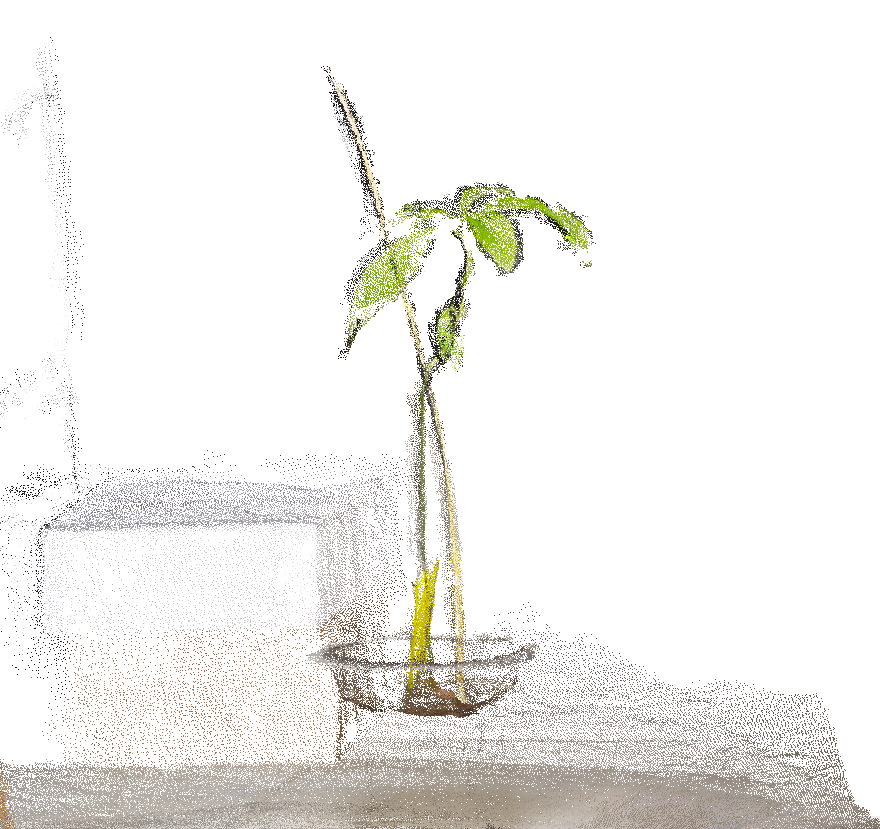
\includegraphics[width=1.0\textwidth]{./Images/PointCloudGeneration_odm.png}
			\caption{ODM}
			\label{fig:odm}
		\end{minipage}\hfill
		\begin{minipage}{0.475\textwidth}
			\centering
			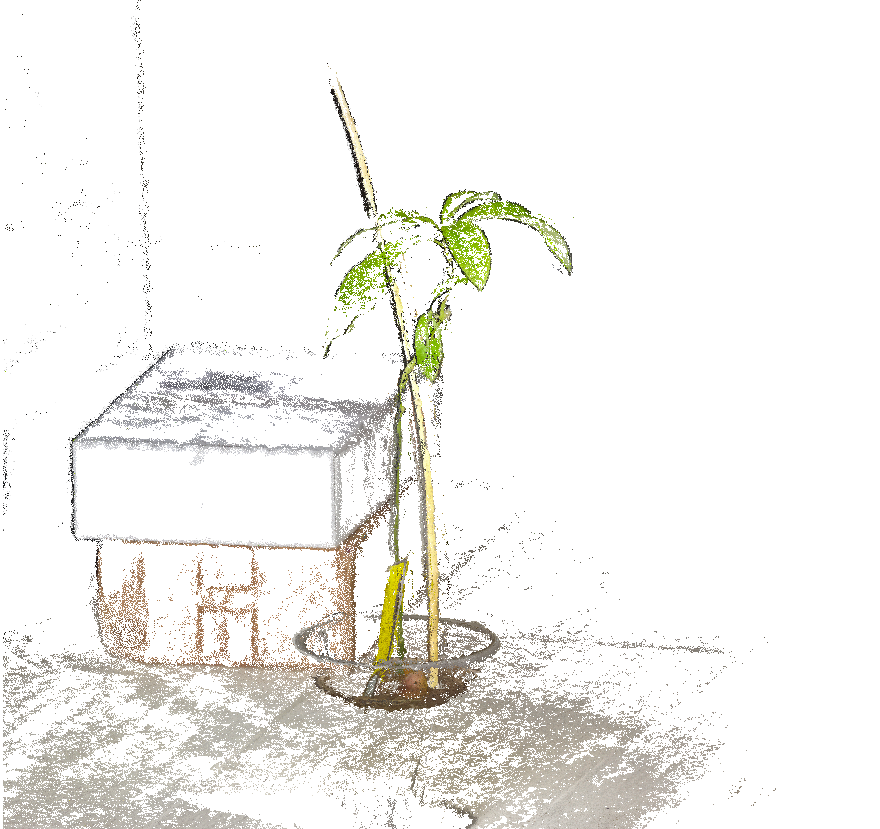
\includegraphics[width=1.0\textwidth]{./Images/PointCloudGeneration_colmap.png}
			\caption{Colmap}
			\label{fig:colmap}
		\end{minipage}
	\end{figure}
}
\frame{
	\frametitle{Generierung von Punktwolken} 
	\begin{figure}
		\centering
		\begin{minipage}{0.3\textwidth}
			\centering
			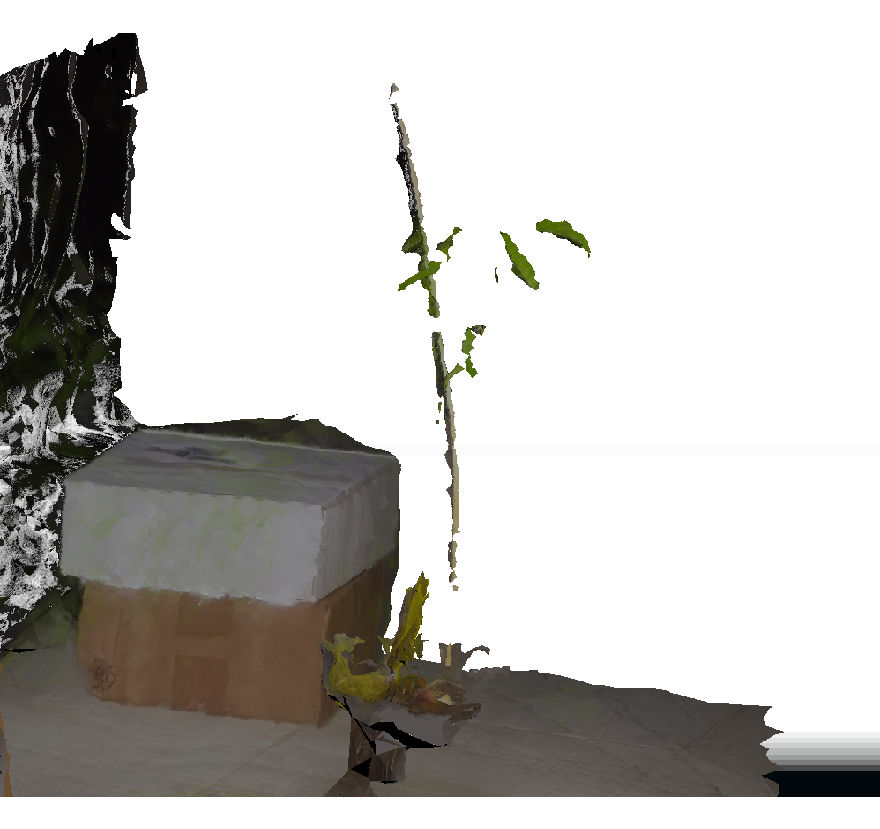
\includegraphics[width=1.0\textwidth]{./Images/PointCloudGeneration_meshroom.png}
			\caption{Meshroom}
			\label{fig:meshroom}
		\end{minipage}\hfill
		\begin{minipage}{0.3\textwidth}
			\centering
			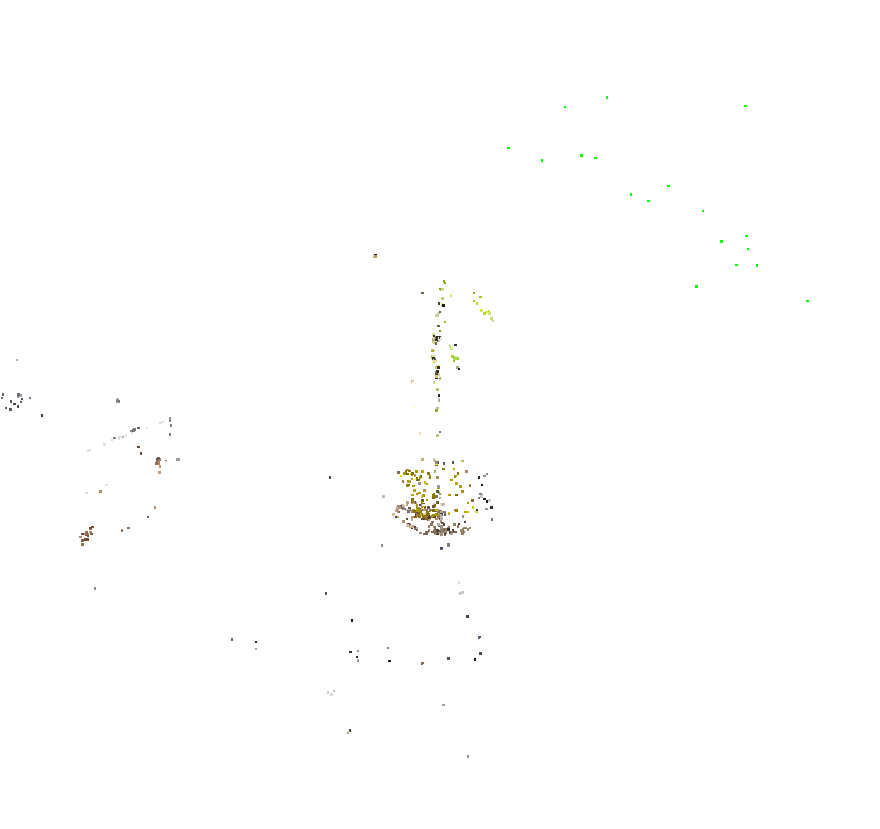
\includegraphics[width=1.0\textwidth]{./Images/PointCloudGeneration_openmvg.png}
			\caption{OpenMVG}
			\label{fig:openmvg}
		\end{minipage}\hfill
		\begin{minipage}{0.3\textwidth}
			\centering
			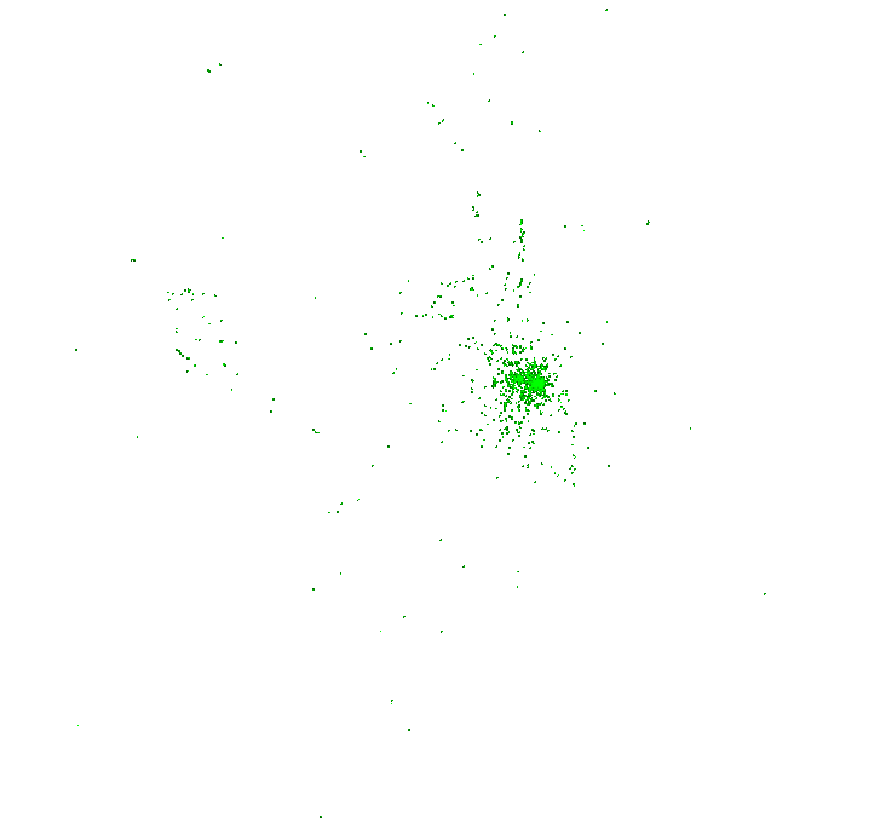
\includegraphics[width=1.0\textwidth]{./Images/PointCloudGeneration_opencv.png}
			\caption{OpenCV}
			\label{fig:opencv}
		\end{minipage}
	\end{figure}
}

\section{Segmentierung}
\frame{
	\frametitle{Segmentierung - Pflanze} 
	\begin{itemize}
		\item Ansatz 1 Entscheidung auf Basis der Krümmung eines Punktes
		\begin{itemize}
			\item Je höher die Krümmung eines Punktes ist desto wahrscheinlicher gehört dieser zu einem Stiel.
			\item Problem: Parametrisierung für alle Pflanzen-Arten
			\item Problem: Blätter haben teilweise ähnlich Krümmung wie Stiele
			\item Problem: Entfernung des Hintergrundes bleibt offen
			\item Nachteil: Binärer Klassifier (Stiel oder nicht Stiel)
		\end{itemize}
		\item Ansatz 2 Nutzen von Neuronalen Netzen (PointNet++)
		\begin{itemize}
			\item Erstellen eines Trainings-Datensatz (144 individuelle Punktwolken + Subsamples)
			\item Training auf diesem Datensatz
			\item Vorteil: Neben Blättern und Stielen können beliebig viele weitere Klassen segmentiert werden. 
			\item Nachteil: Erstellen der Trainings-Daten sehr Zeit aufwendig + Daten müssen verfügbar sein.
		\end{itemize}
	\end{itemize}
}
\frame{
	\frametitle{Segmentierung - Pflanze} 
	\begin{figure}
		\centering
		\begin{minipage}{0.475\textwidth}
			\centering
			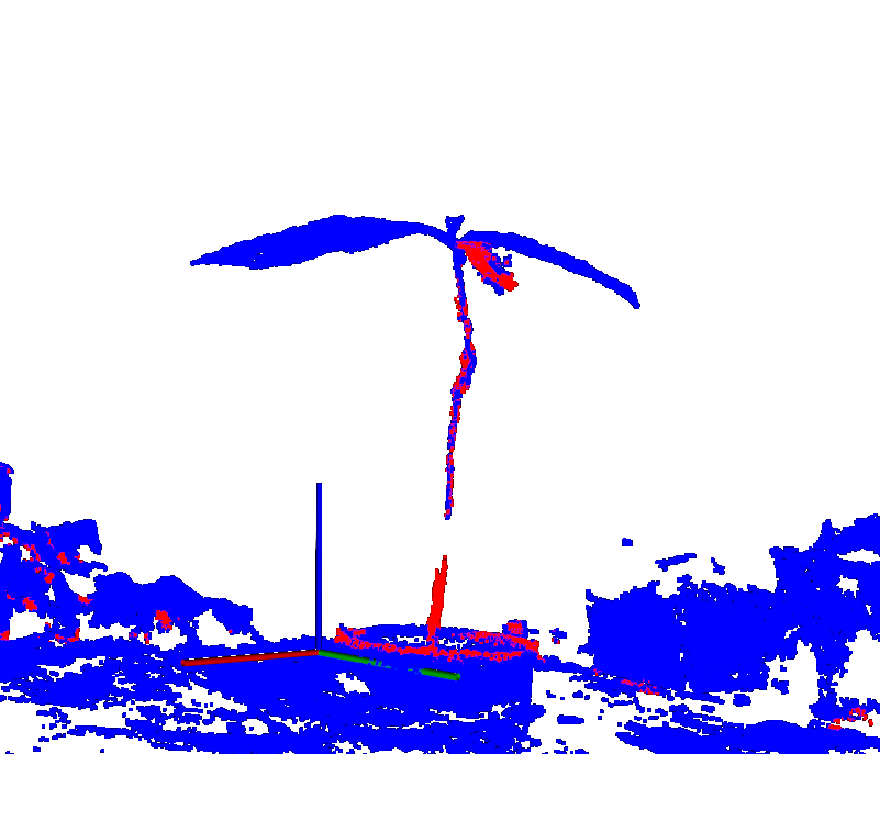
\includegraphics[width=1.0\textwidth]{./Images/HandcraftedClassifierAvocado.png}
			\caption{Avocado Ansatz 1}
			\label{fig:classifier:1}
		\end{minipage}\hfill
		\begin{minipage}{0.475\textwidth}
			\centering
			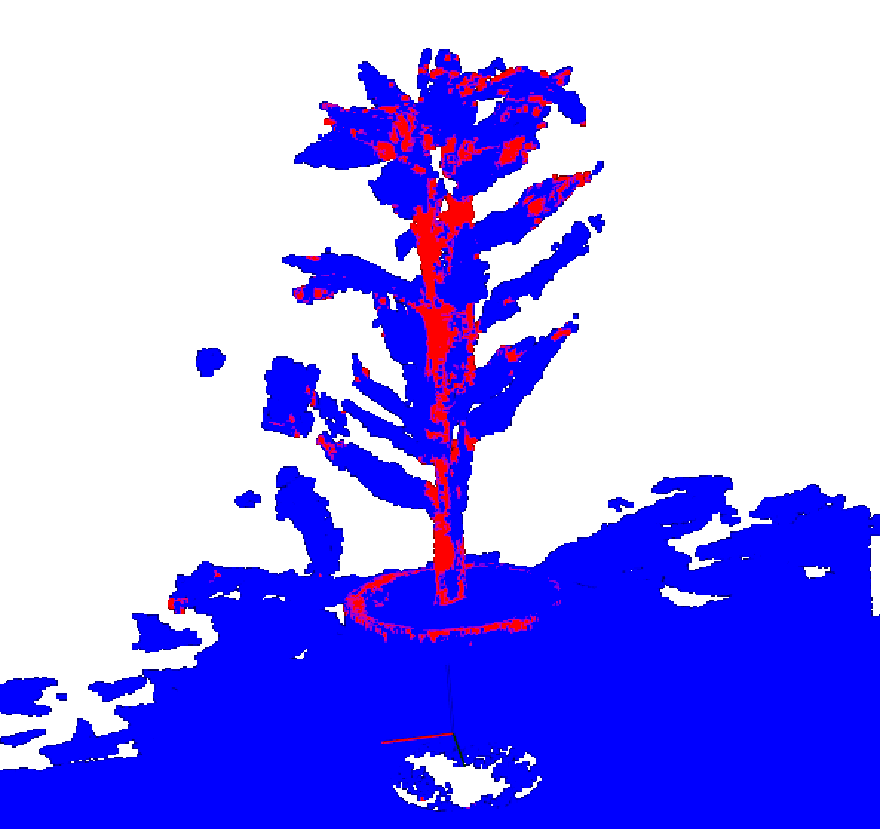
\includegraphics[width=1.0\textwidth]{./Images/HandcraftedClassifierPlant2.png}
			\caption{Plant2 Ansatz 1}
			\label{fig:classifier:2}
		\end{minipage}
	\end{figure}
}
\frame{
	\frametitle{Segmentierung - Pflanze} 
	\begin{figure}
		\centering
		\begin{minipage}{0.475\textwidth}
			\centering
			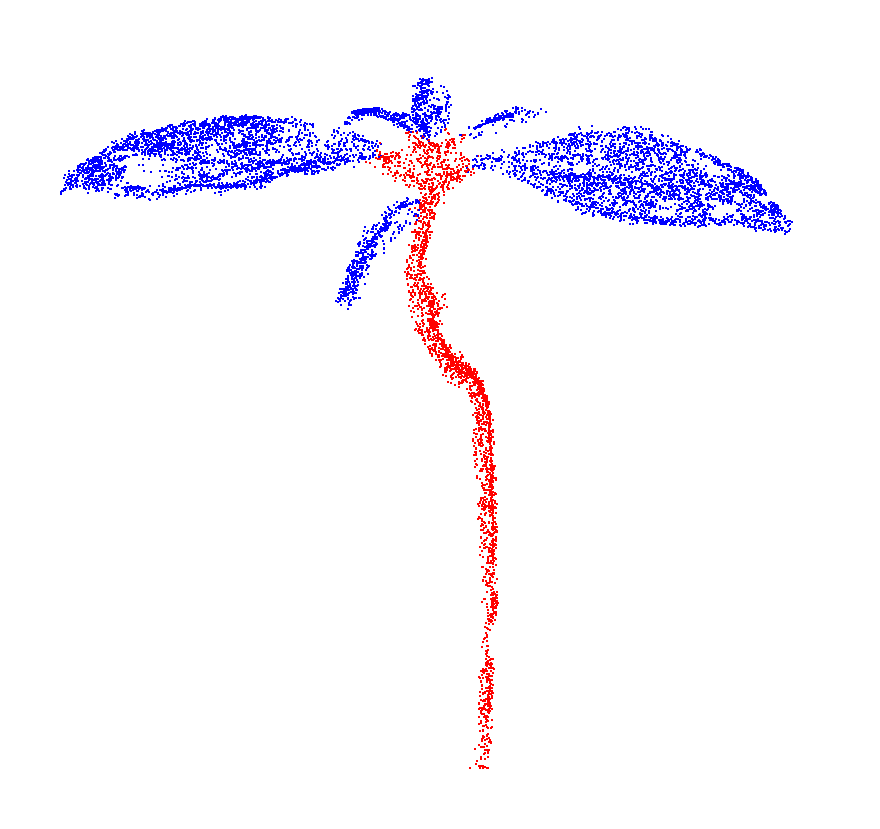
\includegraphics[width=1.0\textwidth]{./Images/Plant_Avocado.png}
			\caption{Avocado Ansatz 2}
			\label{fig:classifier:1}
		\end{minipage}\hfill
		\begin{minipage}{0.475\textwidth}
			\centering
			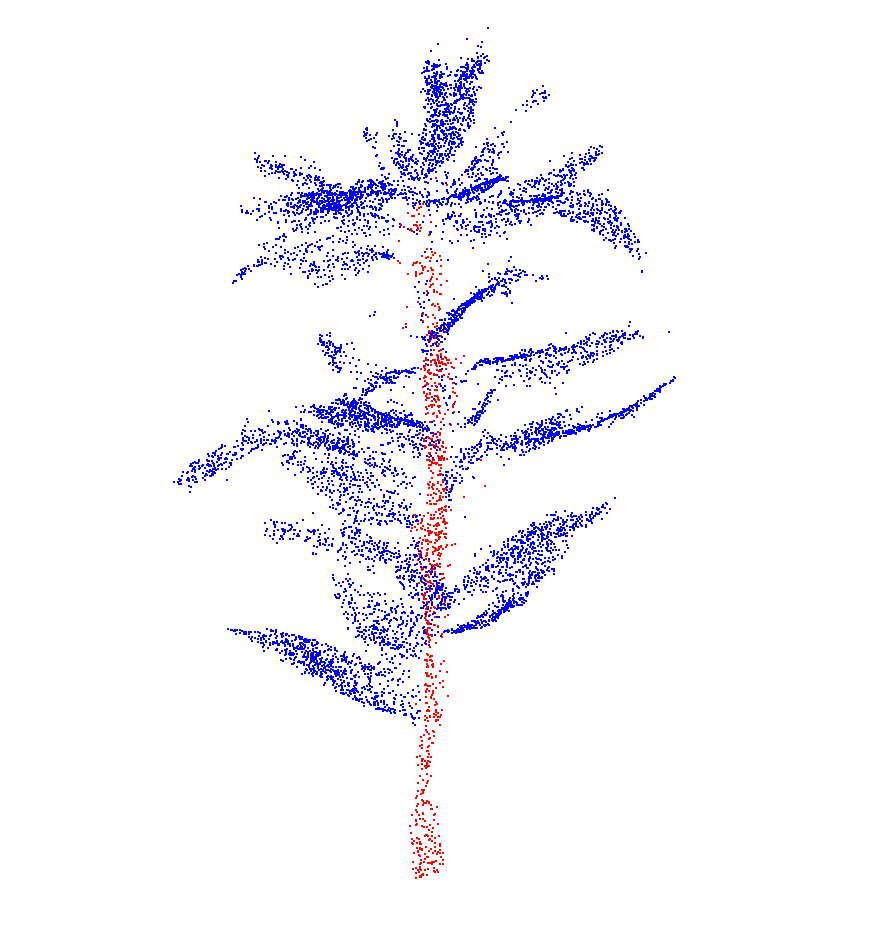
\includegraphics[width=1.0\textwidth]{./Images/Plant_Plant2.png}
			\caption{Plant2 Ansatz 2}
			\label{fig:classifier:2}
		\end{minipage}
	\end{figure}
}
\frame{
	\frametitle{Segmentierung - Hintergrund} 
	\begin{itemize}
		\item Auch hier wurde PointNet++ verwendet.
		\item Ergebnisse sind durch den großen Anteil der Hintergrund-Punkte nicht ideal.
		\item Hier besser eine Szenen-Analyse durchführen und auf Bereichen die als Pflanze erkannt wurde Hintergrund-Segmentierung anwenden um Pflanze freizustellen.
	\end{itemize}
}
\frame{
	\frametitle{Segmentierung - Hintergrund} 
	\begin{figure}
		\centering
		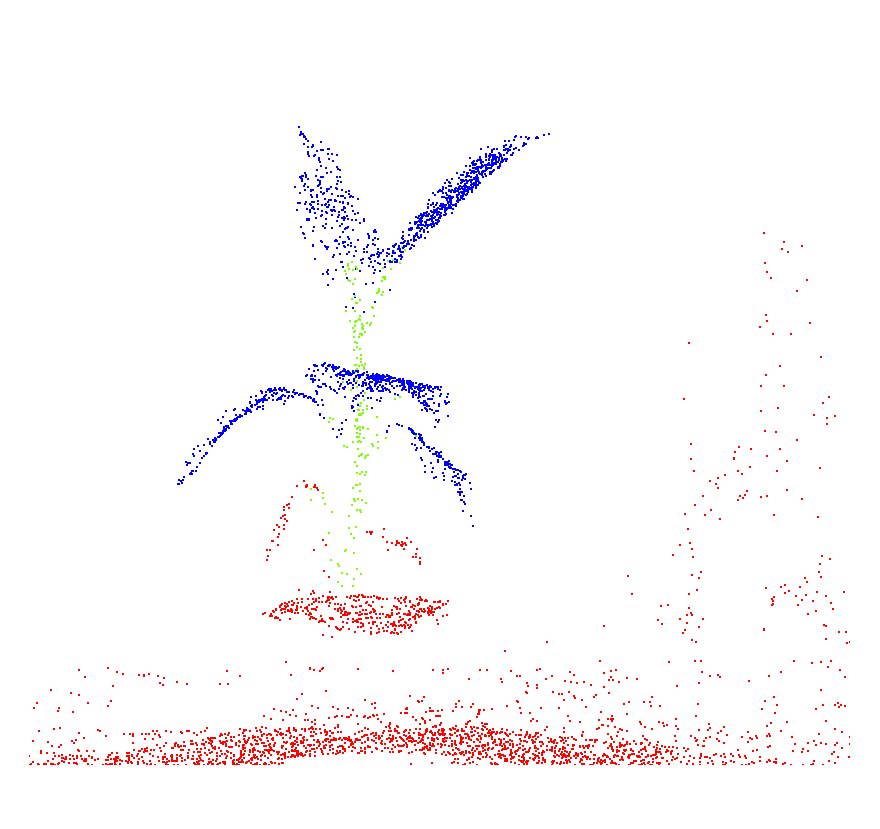
\includegraphics[width=0.65\textwidth]{./Images/BG_Banana.png}
		\caption{Ergebnis Hintergrundsegmentierung}
		\label{fig:background}
	\end{figure}
}
	
\section{Registrierung}
\frame{
	\frametitle{Registrierung} 
	\begin{itemize}
		\item Problem: Da beim Erstellen der Punktwolke mit SfM der Maßstab nicht ermittelt werden kann, liegen verschiedene Punktwolken derselben Szene in unterschiedlichen Maßstäben vor.
		\item Lösung: Daher müssen Punktwolken zu unterschiedlichen Zeitpunkten miteinander registriert werden.
		\item Problem: Die meisten Registrierungsverfahren berücksichtigen nicht die Skalierung.
		\item Es wurden mehrere Ansätze untersucht dieses Problem zu lösen.
		\item Grundgedanke: Punktwolken mit einer Hintergrund-Punktwolke registrieren.
	\end{itemize}
}
\frame{
	\frametitle{Registrierung - ICP mit Schätzung der Skalierung und DCP} 
	\begin{itemize}
		\item In der Bibliothek Point Cloud Libary (PCL) wird eine Implementation die auch einen Wert für die Skalierung liefert bereit gestellt.
		\item Problem: ICP benötigt gute Initialisierung.
		\item Initialisierung finden:
		\begin{itemize}
			\item Punktwolken an der XY-Ebene ausrichten.
			\item Punktwolken auf die selbe Größe bringen.
			\item Bereich um Zentrum entnehmen.
			\item Punktwolken auf die selbe Größe bringen.
			\item Störung herausfiltern
			\item Registrierung mit SIFT-3D
		\end{itemize}
		\item Nach Schätzung der Skalierung Nachverarbeitung.
		\item Problem: Ansatz funktioniert nur bedingt für einige Punktwolken.
	\end{itemize}
}
\frame{
	\frametitle{Registrierung - DCP anpassen} 
	\begin{itemize}
		\item DCP ist ein Neuronales Netz, welches das Registrierungsproblem löst, aber keine Skalierung liefert.
		\item SVD-Head anpassen und Eingabe erweitern.
		\item Resultat des SVD-Head ist nun eine $4 \times 4$ Matrix.
		\item Annahme das diese Matrix als Transformations-Matrix interpretiert werden kann hat sich nicht bestätigt.
	\end{itemize}
}
\frame{
	\frametitle{Registrierung - Iterative Schätzung der Skalierung} 
	\begin{itemize}
		\item Iteratives durchprobieren verschiedener Skalierungen mit anschließender Registrierung.
		\item Für jede Iteration den Abstand der Punktwolke messen und die Iteration wählen, welche den kleinsten Abstand ergab.
		\item Einsatz von verschiedenen Registrierungsverfahren möglich.
		\item Relativ gute Ergebnisse, aber auch hier kommt es immer wieder zu Ausreißern.
	\end{itemize}
}
\frame{
	\frametitle{Registrierung - Iterative Schätzung der Skalierung} 
	\begin{figure}
		\centering
		\begin{minipage}{0.3\textwidth}
			\centering
			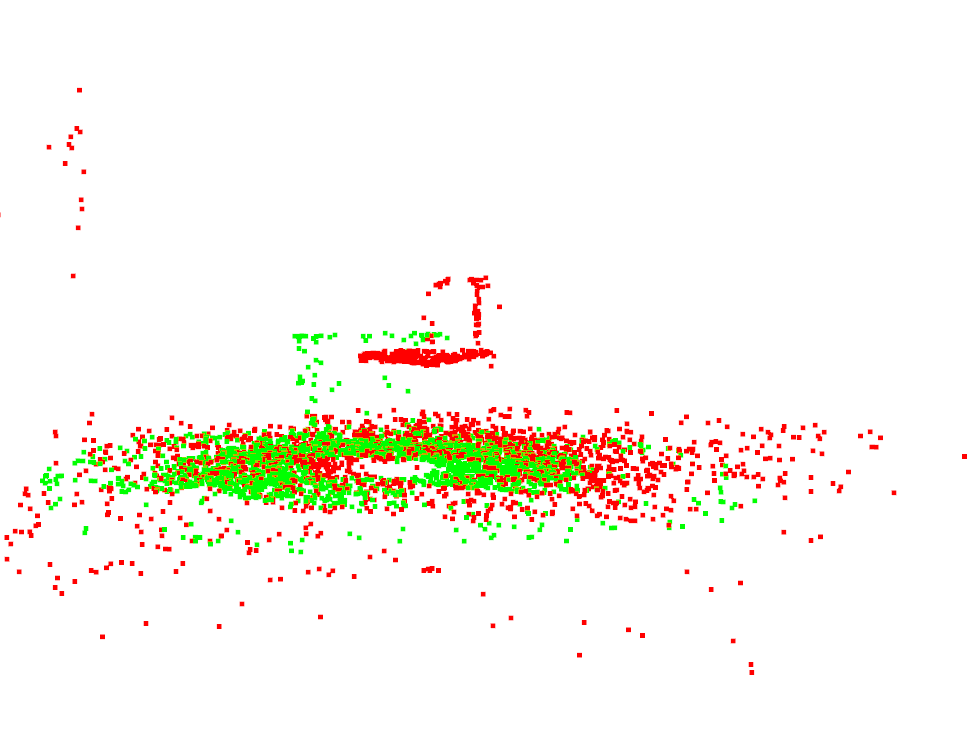
\includegraphics[width=1.0\textwidth]{./Images/RegistrationBananaT1.png}
			\label{fig:meshroom}
		\end{minipage}\hfill
		\begin{minipage}{0.3\textwidth}
			\centering
			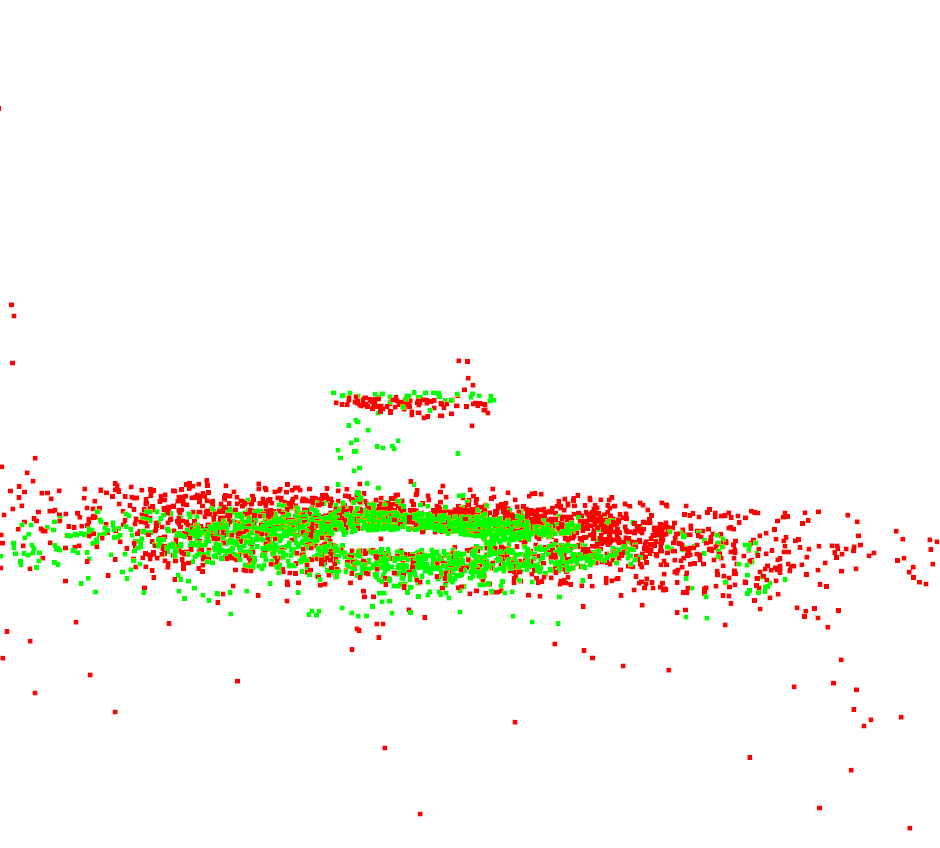
\includegraphics[width=1.0\textwidth]{./Images/RegistrationBananaT2.png}
			\label{fig:openmvg}
		\end{minipage}\hfill
		\begin{minipage}{0.3\textwidth}
			\centering
			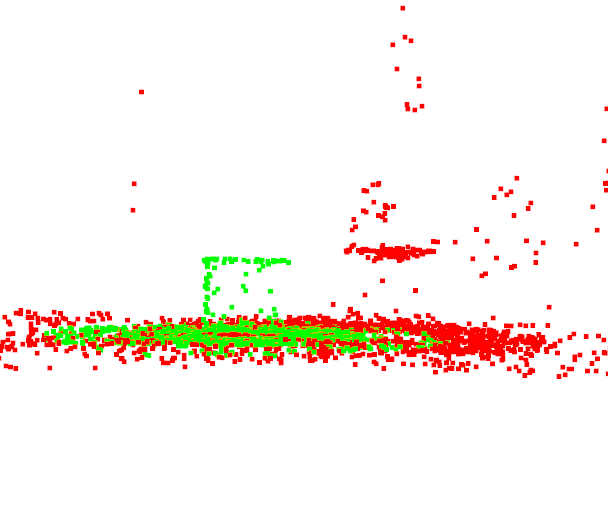
\includegraphics[width=1.0\textwidth]{./Images/RegistrationBananaT3.png}
			\label{fig:opencv}
		\end{minipage}
		\caption{Registrierungsergebnisse für drei Zeitpunkte einer Pflanze}
	\end{figure}
}

\section{Server}
\frame{
	\frametitle{Server} 
	\begin{itemize}
		\item Vier Schnittstellen um Anwendung zu nutzen.
		\begin{itemize}
			\item POST /data/\{Messreihe\}/\{Zeitstempel\}
			\item PUT /data/\{Messreihe\}/\{Zeitstempel\}
			\item GET /listing/\{Messreihe\}
			\item GET /result/\{Messreihe\}/\{Zeitstempel\}
		\end{itemize}
		\item Bearbeitung einzelner Jobs im Hintergrund.
		\item Zugriffe auf geteilte Ressourcen werden über Mutexe geschützt.
	\end{itemize}
}
\frame{
	\frametitle{Pipelines} 
	\begin{figure}
		\centering
		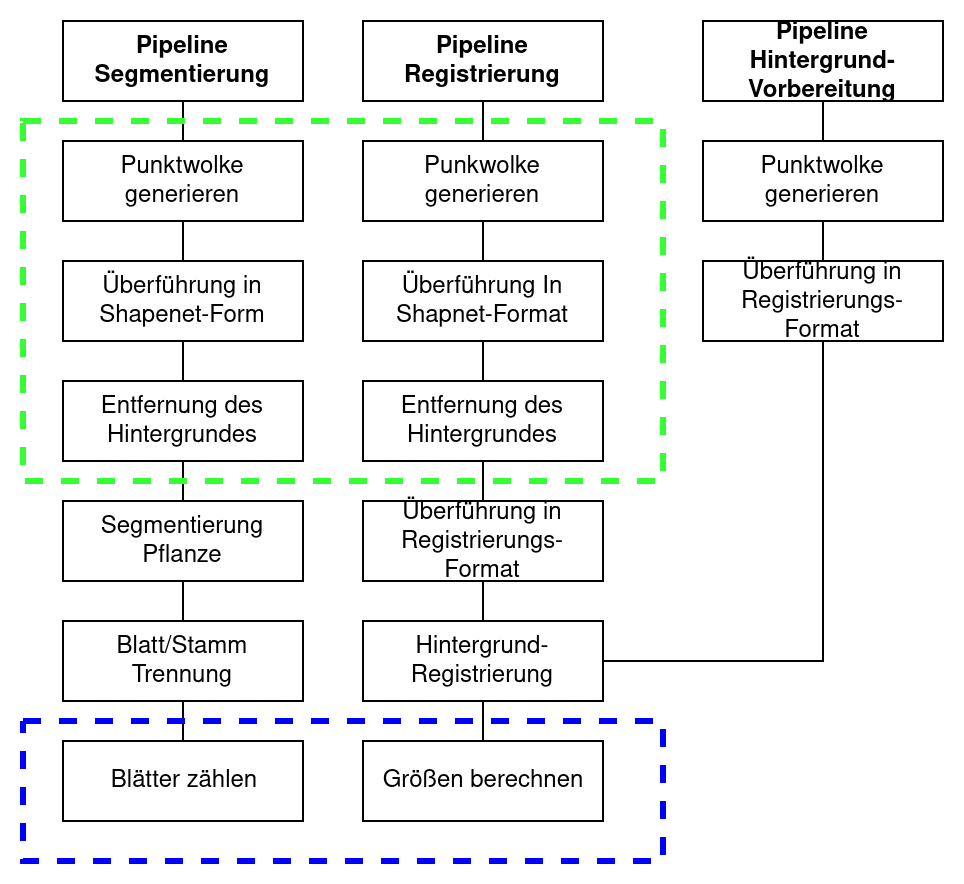
\includegraphics[width=0.65\textwidth]{./Images/Pipelines.png}
		\caption{Übersicht über die einzelnen Pipelines und die darin enthaltenen Jobs.}
		\label{fig:Pipelines}
	\end{figure}
}
\frame{
	\frametitle{Demo} 
	\begin{figure}
		\centering
		\begin{minipage}{0.3\textwidth}
			\centering
			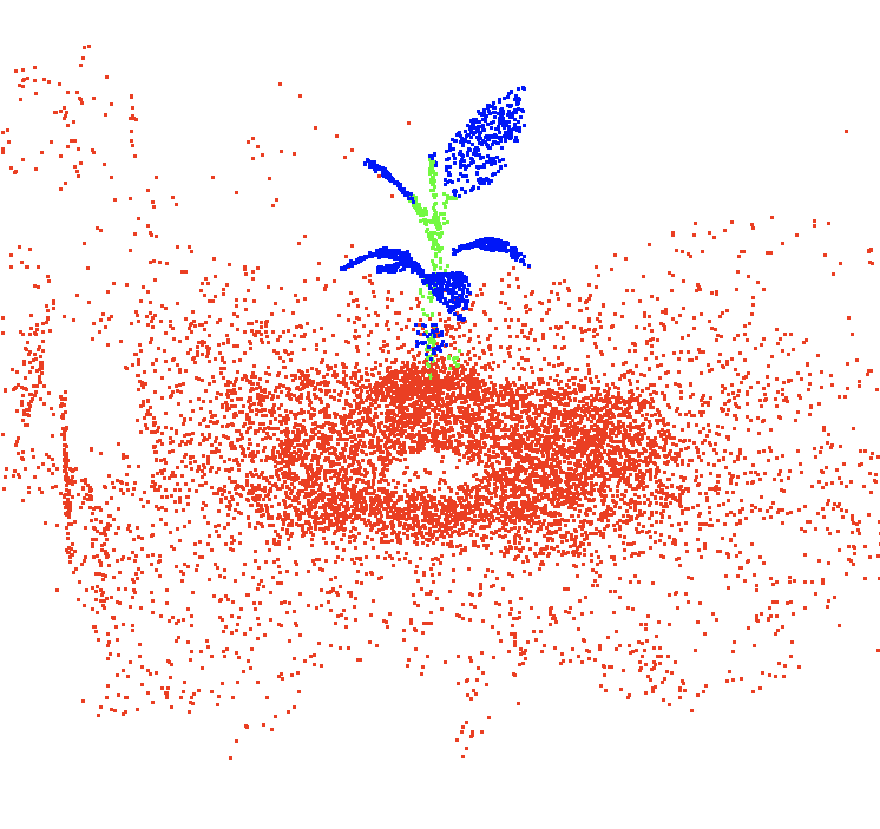
\includegraphics[height=4.5cm,width=4.5cm]{./Images/PipelineBackgroundSegmentationStriped.png}
			\caption{Hintegrund-Segmentierung}
			\label{fig:PiplineBackgroundSegmentation}
		\end{minipage}\hfill
		\begin{minipage}{0.3\textwidth}
			\centering
			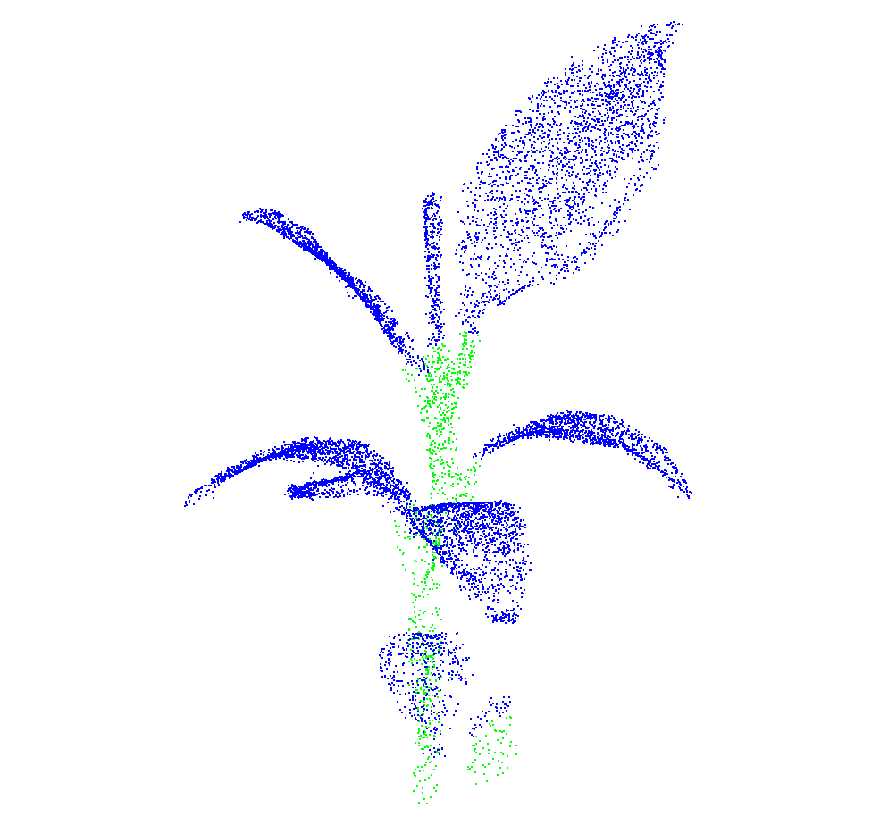
\includegraphics[height=4.5cm,width=4.5cm]{./Images/PipelinePlantSegmentation.png}
			\caption{Planzen-Segmentierung}
			\label{fig:PipelinePlantSegmentation}
		\end{minipage}\hfill
		\begin{minipage}{0.3\textwidth}
			\centering
			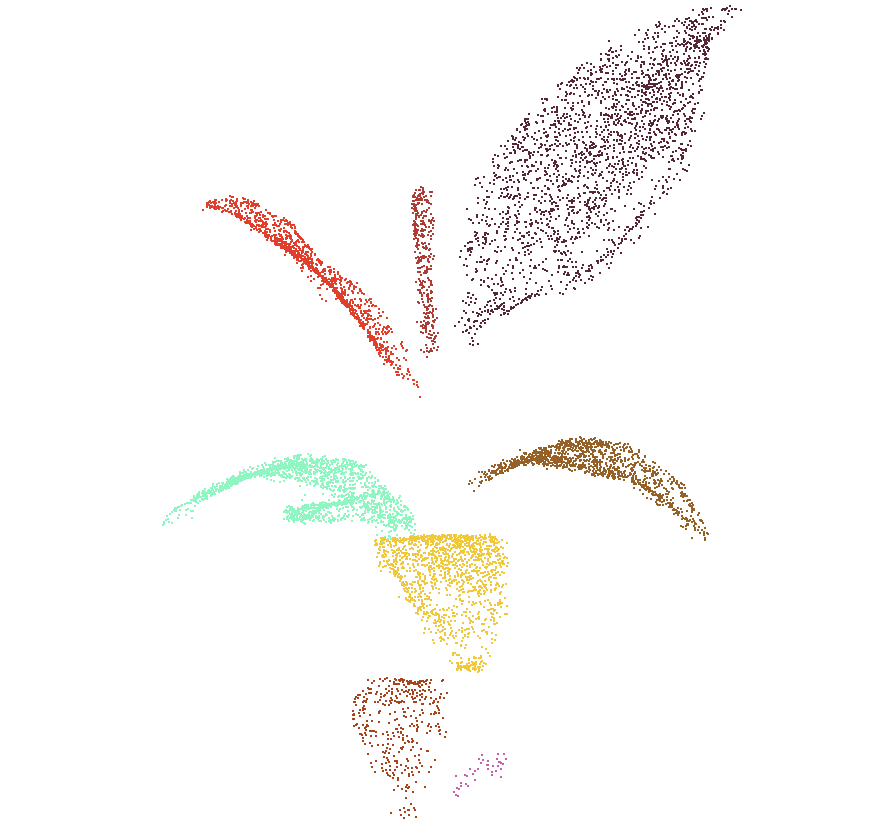
\includegraphics[height=4.5cm,width=4.5cm]{./Images/PipelineLeaveSegmentationStriped.png}
			\caption{Blatt-Segmentierung}
			\label{fig:PipelineLeaveSegmentation}
		\end{minipage}
	\end{figure}
}

\section{Quellen}
\begin{frame}[allowframebreaks]
    \frametitle{Referenzen}
    \bibliographystyle{ieeetr}
    \bibliography{./bibleografie.bib}
\end{frame}

\end{document}
